\documentclass[portrait,final,a0paper,fontscale=0.277]{baposter}

\usepackage{listings}

\usepackage{calc}
\usepackage{graphicx}
\usepackage{amsmath}
\usepackage{amssymb}
\usepackage{relsize}
\usepackage{multirow}
\usepackage{rotating}
\usepackage{bm}
\usepackage{url}

\usepackage{graphicx}
\usepackage{multicol}

%\usepackage{times}
%\usepackage{helvet}
%\usepackage{bookman}
\usepackage{palatino}

\usepackage{xspace}

\usepackage{listings}

\lstset{ %
language=Java,                % choose the language of the code
columns=flexible,
lineskip=-1pt,
basicstyle=\ttfamily\small,       % the size of the fonts that are used for the code
numbers=none,                   % where to put the line-numbers
numberstyle=\ttfamily\tiny,      % the size of the fonts that are used for the line-numbers
stepnumber=1,                   % the step between two line-numbers. If it's 1 each line will be numbered
numbersep=5pt,                  % how far the line-numbers are from the code
backgroundcolor=\color{white},  % choose the background color. You must add \usepackage{color}
showspaces=false,               % show spaces adding particular underscores
showstringspaces=false,         % underline spaces within strings
showtabs=false,                 % show tabs within strings adding particular underscores
morekeywords={var},
%  frame=single,                   % adds a frame around the code
tabsize=2,                  % sets default tabsize to 2 spaces
captionpos=none,                   % sets the caption-position to bottom
breaklines=true,                % sets automatic line breaking
breakatwhitespace=false,        % sets if automatic breaks should only happen at whitespace
title=\lstname,                 % show the filename of files included with \lstinputlisting; also try caption instead of title
escapeinside={(*}{*)},          % if you want to add a comment within your code
keywordstyle=\ttfamily\bfseries,
aboveskip=0pt,
belowskip=0pt,
frame=single %border
% commentstyle=\color{Gray},
% stringstyle=\color{Green}
}


\newcommand{\captionfont}{\footnotesize}

\graphicspath{{images/}{../images/}}
\usetikzlibrary{calc}

\newcommand{\SET}[1]  {\ensuremath{\mathcal{#1}}}
\newcommand{\MAT}[1]  {\ensuremath{\boldsymbol{#1}}}
\newcommand{\VEC}[1]  {\ensuremath{\boldsymbol{#1}}}
\newcommand{\Video}{\SET{V}}
\newcommand{\video}{\VEC{f}}
\newcommand{\track}{x}
\newcommand{\Track}{\SET T}
\newcommand{\LMs}{\SET L}
\newcommand{\lm}{l}
\newcommand{\PosE}{\SET P}
\newcommand{\posE}{\VEC p}
\newcommand{\negE}{\VEC n}
\newcommand{\NegE}{\SET N}
\newcommand{\Occluded}{\SET O}
\newcommand{\occluded}{o}
\newcommand\mixin{\textbf{\texttt{@Obj }}}

%%%%%%%%%%%%%%%%%%%%%%%%%%%%%%%%%%%%%%%%%%%%%%%%%%%%%%%%%%%%%%%%%%%%%%%%%%%%%%%%
%%%% Some math symbols used in the text
%%%%%%%%%%%%%%%%%%%%%%%%%%%%%%%%%%%%%%%%%%%%%%%%%%%%%%%%%%%%%%%%%%%%%%%%%%%%%%%%

%%%%%%%%%%%%%%%%%%%%%%%%%%%%%%%%%%%%%%%%%%%%%%%%%%%%%%%%%%%%%%%%%%%%%%%%%%%%%%%%
% Multicol Settings
%%%%%%%%%%%%%%%%%%%%%%%%%%%%%%%%%%%%%%%%%%%%%%%%%%%%%%%%%%%%%%%%%%%%%%%%%%%%%%%%
\setlength{\columnsep}{1.5em}
\setlength{\columnseprule}{0mm}

%%%%%%%%%%%%%%%%%%%%%%%%%%%%%%%%%%%%%%%%%%%%%%%%%%%%%%%%%%%%%%%%%%%%%%%%%%%%%%%%
% Save space in lists. Use this after the opening of the list
%%%%%%%%%%%%%%%%%%%%%%%%%%%%%%%%%%%%%%%%%%%%%%%%%%%%%%%%%%%%%%%%%%%%%%%%%%%%%%%%
\newcommand{\compresslist}{%
\setlength{\itemsep}{0pt}%
\setlength{\parskip}{0pt}%
\setlength{\parsep}{0pt}%
}

\newcommand{\documentcollection}{D}
\newcommand{\paper}{d}
\newcommand{\milestonepaperset}{M}
\newcommand{\object}{O}
\newcommand{\objectvar}{o}
\newcommand{\probability}{p}
\newcommand{\topicset}{T}
\newcommand{\authorset}{A}
\newcommand{\venueset}{V}
\newcommand{\papers}{P}
\newcommand{\citationvar}{c}
\newcommand{\citationset}{C}
\newcommand{\citingpaper}{CD}
\newcommand{\cpmatrix}{N}
\newcommand{\camatrix}{U}
\newcommand{\cvmatrix}{E}
\newcommand{\topic}{z}
\newcommand{\authorvar}{a}
\newcommand{\venue}{v}
\newcommand{\topicdis}{\phi}
\newcommand{\parameters}{\theta}
\newcommand{\likelihood}{L}
\newcommand{\topicnumber}{k}

\newcommand{\offcommitteeset}{\overline{\committeeset}}
\newcommand{\expertset}{E}
\newcommand{\yearvar}{y}
\newcommand{\yearset}{Y}
\newcommand{\yearintervalhalf}{h}
\newcommand{\yearintervalhalfbefore}{h_b}
\newcommand{\yearintervalhalfafter}{h_a}
\newcommand{\yearbegin}{\yearvar_i}
\newcommand{\yearend}{\yearvar_o}


\newcommand{\union}{\bigcup}
\newcommand{\intersection}{\bigcap}
\newcommand{\papervar}{q}
\newcommand{\paperset}{Q}
\newcommand{\paperauthorcount}{n}
\newcommand{\papercommitteeauthorcount}{m}

\newcommand{\technicalscore}{\tau}
\newcommand{\politicalscore}{\psi}
\newcommand{\paperscore}{\varrho}
\newcommand{\paperscorefunc}{\Upsilon}
\newcommand{\randomvar}{\varepsilon}

\newcommand{\expertpopulation}{x}
\newcommand{\committeepopulation}{z}

\newcommand{\probabilityvar}{P}
\newcommand{\setsize}[1]{\|#1\|}
\newcommand{\normalizedsetsize}[1]{\|#1\|^{\ast}}
\newcommand{\combination}{\mathrm{C}}
\newcommand{\numberset}{B}
\newcommand{\numbervar}{b}
\newcommand{\yearintervalhalfset}{H}
\newcommand{\conferencevar}{c}
\newcommand{\threshold}{T}
\newcommand{\nomore}{\mathrm{\leq}}
\newcommand{\noless}{\mathrm{\geq}}
\newcommand{\boudaryyearset}{Y_{B}}
\newcommand{\boudaryyearvar}{\yearvar_b}
\newcommand{\upboudaryyearset}{Y_{up}}
\newcommand{\bottomboudaryyearset}{Y_{bottom}}
\newcommand{\firstcondition}{F_1}
\newcommand{\secondcondition}{F_2}
\newcommand{\thirdcondition}{F_3}
\newcommand{\nodifference}{\overline{D}}
\newcommand{\appropriateh}{\yearintervalhalf'}
\newcommand{\e}{\mathrm{e}}
\newcommand{\normalizedgroup}{N}
\newcommand{\comparedgroup}{Z}
\newcommand{\correspondinggroup}{z}
\newcommand{\etasquare}{\eta^2}
\newcommand{\paperexpertcount}{e}
\newcommand{\coauthorvar}{c}

%eliminate
\newcommand{\sizeset}{s}%eliminate
\newcommand{\cardinality}{Ca}%eliminate
\newcommand{\technicalvar}{pt}
\newcommand{\politicalvar}{ps}
\newcommand{\papertechnicalvar}{Ppt}
\newcommand{\paperpoliticalvar}{Pps}
\newcommand{\statusvar}{S}
\newcommand{\modelvar}{M}
\newcommand{\regionvar}{R}

\newcommand{\avg}{\mathrm{avg}}

\newcommand{\rejectnull}{$\times$}
\newcommand{\acceptnull}{$\surd$}
\newcommand{\remarknull}{$*$}

\newcommand{\comp}{\upsilon}

%%%%%%%%%%%%%%%%%%%%%%%%%%%%%%%%%%%%%%%%%%%%%%%%%%%%%%%%%%%%%%%%%%%%%%%%%%%%%%
%%% Begin of Document
%%%%%%%%%%%%%%%%%%%%%%%%%%%%%%%%%%%%%%%%%%%%%%%%%%%%%%%%%%%%%%%%%%%%%%%%%%%%%%

\begin{document}

%%%%%%%%%%%%%%%%%%%%%%%%%%%%%%%%%%%%%%%%%%%%%%%%%%%%%%%%%%%%%%%%%%%%%%%%%%%%%%
%%% Here starts the poster
%%%---------------------------------------------------------------------------
%%% Format it to your taste with the options
%%%%%%%%%%%%%%%%%%%%%%%%%%%%%%%%%%%%%%%%%%%%%%%%%%%%%%%%%%%%%%%%%%%%%%%%%%%%%%
% Define some colors

%\definecolor{lightblue}{cmyk}{0.83,0.24,0,0.12}
\definecolor{lightblue}{rgb}{0.145,0.6666,1}

% Draw a video
\newlength{\FSZ}
\newcommand{\drawvideo}[3]{% [0 0.25 0.5 0.75 1 1.25 1.5]
   \noindent\pgfmathsetlength{\FSZ}{\linewidth/#2}
   \begin{tikzpicture}[outer sep=0pt,inner sep=0pt,x=\FSZ,y=\FSZ]
   \draw[color=lightblue!50!black] (0,0) node[outer sep=0pt,inner sep=0pt,text width=\linewidth,minimum height=0] (video) {\noindent#3};
   \path [fill=lightblue!50!black,line width=0pt]
     (video.north west) rectangle ([yshift=\FSZ] video.north east)
    \foreach \x in {1,2,...,#2} {
      {[rounded corners=0.6] ($(video.north west)+(-0.7,0.8)+(\x,0)$) rectangle +(0.4,-0.6)}
    }
;
   \path [fill=lightblue!50!black,line width=0pt]
     ([yshift=-1\FSZ] video.south west) rectangle (video.south east)
    \foreach \x in {1,2,...,#2} {
      {[rounded corners=0.6] ($(video.south west)+(-0.7,-0.2)+(\x,0)$) rectangle +(0.4,-0.6)}
    }
;
   \foreach \x in {1,...,#1} {
     \draw[color=lightblue!50!black] ([xshift=\x\linewidth/#1] video.north west) -- ([xshift=\x\linewidth/#1] video.south west);
   }
   \foreach \x in {0,#1} {
     \draw[color=lightblue!50!black] ([xshift=\x\linewidth/#1,yshift=1\FSZ] video.north west) -- ([xshift=\x\linewidth/#1,yshift=-1\FSZ] video.south west);
   }
   \end{tikzpicture}
}

\hyphenation{resolution occlusions}
%%
\begin{poster}%
  % Poster Options
  {
  % Show grid to help with alignment
  grid=false,
  % Column spacing
  colspacing=0.5em,
  % Color style
  bgColorOne=white,
  bgColorTwo=white,
  borderColor=lightblue,
  headerColorOne=black,
  headerColorTwo=lightblue,
  headerFontColor=white,
  boxColorOne=white,
  boxColorTwo=lightblue,
  % Format of textbox
  textborder=roundedleft,
  % Format of text header
  eyecatcher=true,
  headerborder=closed,
  headerheight=0.1\textheight,
%  textfont=\sc, An example of changing the text font
  headershape=roundedright,
  headershade=shadelr,
  headerfont=\Large\bf\textsc, %Sans Serif
  textfont={\setlength{\parindent}{1.5em}},
  boxshade=plain,
%  background=shade-tb,
  background=plain,
  linewidth=2pt
  }
  % Eye Catcher
  {
\includegraphics[height=7em]{pdfs/hku.png}}
  % Title
  {\bf\textsc{Classless Java: Interface-based Programming for the Masses}\vspace{0.1em}}
  % Authors
  {\text{Yanlin Wang {,} Haoyuan Zhang {,} Marco Servetto {,} Bruno C. d. S. Oliveira}}
  % \text{The University of Hong Kong, China}}
  % \text{The University of Hong Kong, China: \{ylwang,hyzhang,bruno\}@cs.hku.hk}\\
  % \text{Victoria University of Wellington, New Zealand: marco.servetto@ecs.vuw.ac.nz}}
  % University logo
  {% The makebox allows the title to flow into the logo, this is a hack because of the L shaped logo.
    
\includegraphics[width=7em,height=7em]{pdfs/vuw.png}
  }




%%%%%%%%%%%%%%%%%%%%%%%%%%%%%%%%%%%%%%%%%%%%%%%%%%%%%%%%%%%%%%%%%%%%%%%%%%%%%%
%%% Now define the boxes that make up the poster
%%%---------------------------------------------------------------------------
%%% Each box has a name and can be placed absolutely or relatively.
%%% The only inconvenience is that you can only specify a relative position
%%% towards an already declared box. So if you have a box attached to the
%%% bottom, one to the top and a third one which should be in between, you
%%% have to specify the top and bottom boxes before you specify the middle
%%% box.
%%%%%%%%%%%%%%%%%%%%%%%%%%%%%%%%%%%%%%%%%%%%%%%%%%%%%%%%%%%%%%%%%%%%%%%%%%%%%%
    %
    % A coloured circle useful as a bullet with an adjustably strong filling
    \newcommand{\colouredcircle}{%
      \tikz{\useasboundingbox (-0.2em,-0.32em) rectangle(0.2em,0.32em); \draw[draw=black,fill=lightblue,line width=0.03em] (0,0) circle(0.18em);}}

%%%%%%%%%%%%%%%%%%%%%%%%%%%%%%%%%%%%%%%%%%%%%%%%%%%%%%%%%%%%%%%%%%%%%%%%%%%%%%
  \headerbox{Motivation}{name=motivation,column=0,row=0}{
%%%%%%%%%%%%%%%%%%%%%%%%%%%%%%%%%%%%%%%%%%%%%%%%%%%%%%%%%%%%%%%%%%%%%%%%%%%%%%
   
  \noindent \begin{enumerate}\compresslist
      \item Multiple inheritance with state is hard. 
      \noindent \begin{itemize}\compresslist
        \item Trait is a nice  model but without state.
        \item Multiple inheritance in C++ is complex. Scala traits have fields but no constructors.
        \item Java supports multiple inheritance with default methods in a limited way.
      \end{itemize}
      \item Fields usually cannot be type-refined, which prevents easy solutions to the Expression Problem.
      % 
      % \item Other models (traits, mixins, etc) have certain limitations.
      % \item Our approach is related with traits. But we use operations on state to simulate fields 
      % which traits do not support.
   \end{enumerate}
 }

%%%%%%%%%%%%%%%%%%%%%%%%%%%%%%%%%%%%%%%%%%%%%%%%%%%%%%%%%%%%%%%%%%%%%%%%%%%%%%
  \headerbox{Contributions}{name=contribution,column=0,below=motivation}{
%%%%%%%%%%%%%%%%%%%%%%%%%%%%%%%%%%%%%%%%%%%%%%%%%%%%%%%%%%%%%%%%%%%%%%%%%%%%%%
  \noindent \begin{enumerate}\compresslist
  \item Abstract state operations: 
      \noindent \begin{itemize} \compresslist
          \item a new way to think about state, via operations instead of fields directly
          \item easy to combine with \emph{multiple (trait) inheritance}
          \item supports constructors, co-variant type-refinement of state
      \end{itemize}    
  % \item Classless Java: a Java extension that allows an interface-based programming style
    % \item IB and Object Interfaces: enable powerful programming idioms using multiple-inheritance, type-refinement and abstract state operations.
    \item Classless Java: a practical realization of IB in Java.
    % \item Type-safe covariant mutable state
    % \item Applications and case studies
   \end{enumerate}
   \vspace{0.3em}
  }

  
%%%%%%%%%%%%%%%%%%%%%%%%%%%%%%%%%%%%%%%%%%%%%%%%%%%%%%%%%%%%%%%%%%%%%%%%%%%%%%
  \headerbox{Implementation}{name=implementation,column=0,below=contribution}{
%%%%%%%%%%%%%%%%%%%%%%%%%%%%%%%%%%%%%%%%%%%%%%%%%%%%%%%%%%%%%%%%%%%%%%%%%%%%%%
  
Java supports compilation agents, where Java libraries can interact with the Java compilation process,
acting as a man in the middle between the
generation of AST and bytecode.

This process is facilitated by frameworks like Lombok:
a Java library that aims at reducing Java boilerplate code via
annotations. \mixin was created using Lombok.

\noindent{\centering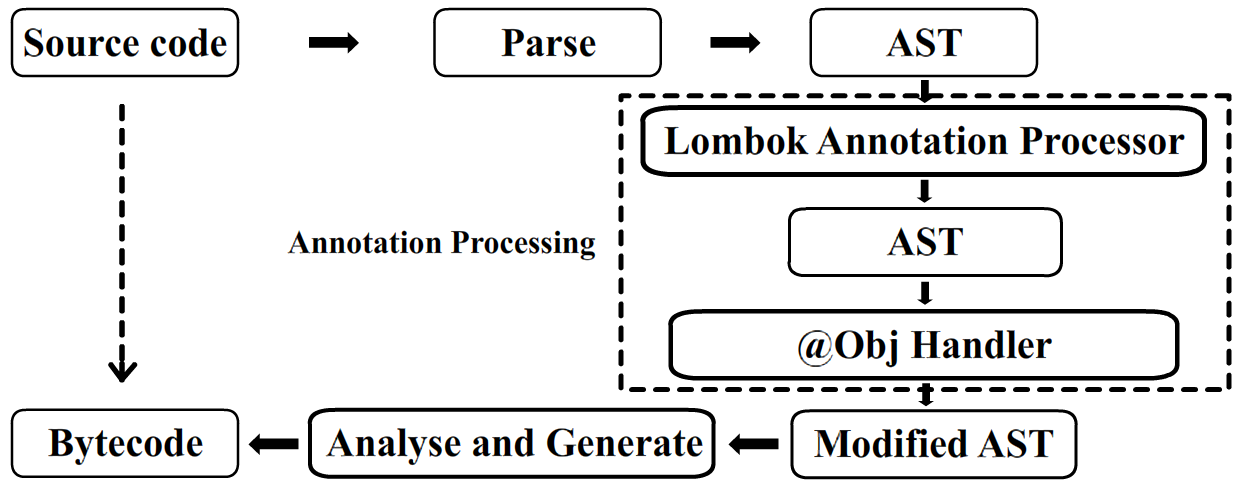
\includegraphics[width=\linewidth]{pdfs/lombok3.png}\\}
\vspace{0.1em}
}


  
%%%%%%%%%%%%%%%%%%%%%%%%%%%%%%%%%%%%%%%%%%%%%%%%%%%%%%%%%%%%%%%%%%%%%%%%%%%%%%
  \headerbox{UML Diagram}{name=uml,column=0,below=implementation}{
%%%%%%%%%%%%%%%%%%%%%%%%%%%%%%%%%%%%%%%%%%%%%%%%%%%%%%%%%%%%%%%%%%%%%%%%%%%%%%
\noindent{\centering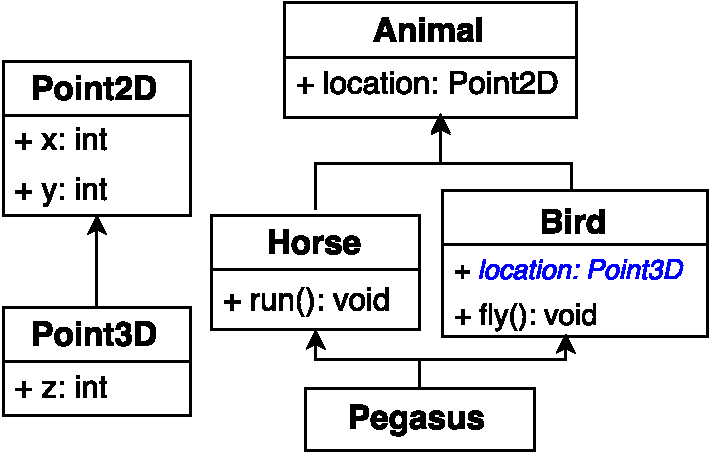
\includegraphics[width=0.8\linewidth]{pdfs/PegasusDetail.pdf}\\}
\vspace{0.1em}
}


  
%%%%%%%%%%%%%%%%%%%%%%%%%%%%%%%%%%%%%%%%%%%%%%%%%%%%%%%%%%%%%%%%%%%%%%%%%%%%%%
  \headerbox{Results (Partial)}{name=result,column=0,below=uml,above=bottom}{
%%%%%%%%%%%%%%%%%%%%%%%%%%%%%%%%%%%%%%%%%%%%%%%%%%%%%%%%%%%%%%%%%%%%%%%%%%%%%%
In the maze game case study, both SLOC and \# of interfaces are greatly reduced:
\noindent{\centering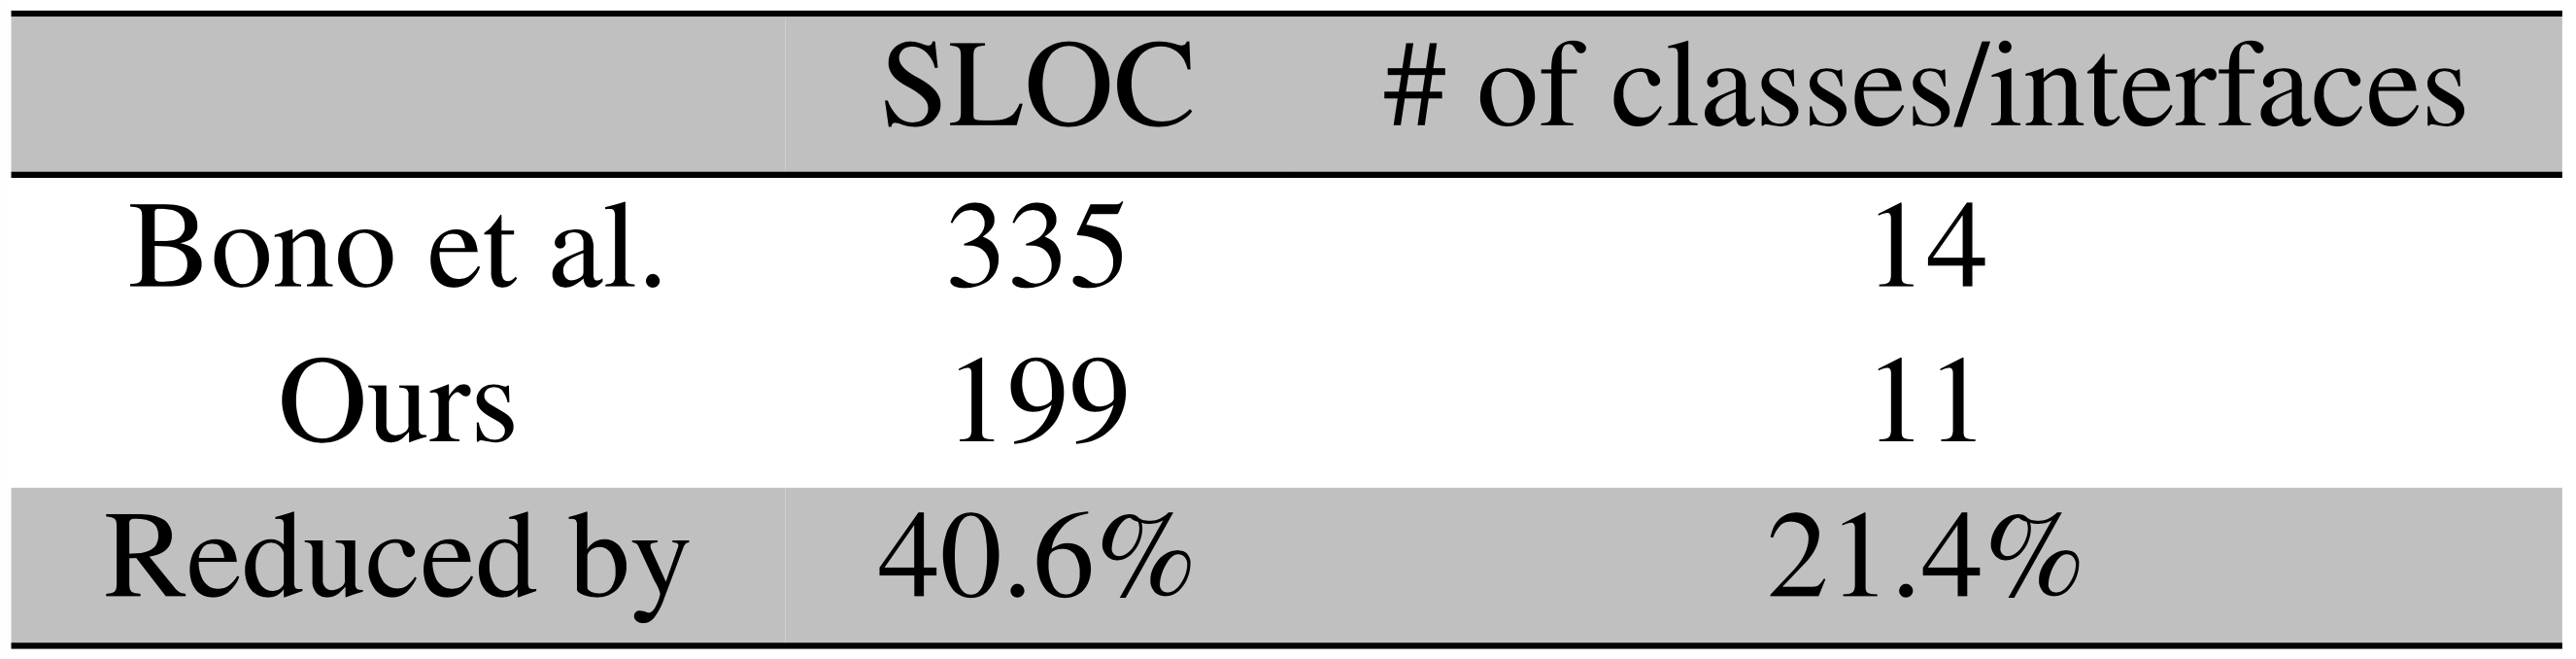
\includegraphics[width=0.81\linewidth]{pdfs/result.png}\\}
\vspace{0.1em}
}


\vspace{-0.5em}
%%%%%%%%%%%%%%%%%%%%%%%%%%%%%%%%%%%%%%%%%%%%%%%%%%%%%%%%%%%%%%%%%%%%%%%%%%%%%%
\headerbox{Object Interfaces and Instantiation}{name=Model,column=1,span=2,row=0}{
  %%%%%%%%%%%%%%%%%%%%%%%%%%%%%%%%%%%%%%%%%%%%%%%%%%%%%%%%%%%%%%%%%%%%%%%%%%%%%%
% \lstinputlisting[linerange=6-13]{../UseMixinLombok/src/pegasus/simple/java8/Main.java}% APPLY:linerange=PEGASUS_JAVA
% \lstinputlisting[linerange=17-19]{../UseMixinLombok/src/pegasus/simple/java8/Main.java}% APPLY:linerange=PEGASUS_INST
\lstinputlisting[linerange=8-12]{../UseMixinLombok/src/pegasus/simple/lombok/Main.java}% APPLY:linerange=PEGASUS_LOMBOK
\lstinputlisting[linerange=1-5]{./import_src/src1.txt}
}

\vspace{-0.5em}
%%%%%%%%%%%%%%%%%%%%%%%%%%%%%%%%%%%%%%%%%%%%%%%%%%%%%%%%%%%%%%%%%%%%%%%%%%%
\headerbox{Object Interfaces with State (immutable data)}{name=results,column=1,span=2,row=0,below=Model}{
  %%%%%%%%%%%%%%%%%%%%%%%%%%%%%%%%%%%%%%%%%%%%%%%%%%%%%%%%%%%%%%%%%%%%%%%%%%%%%%
%  \begin{multicols}{2}
%  \noindent{\centering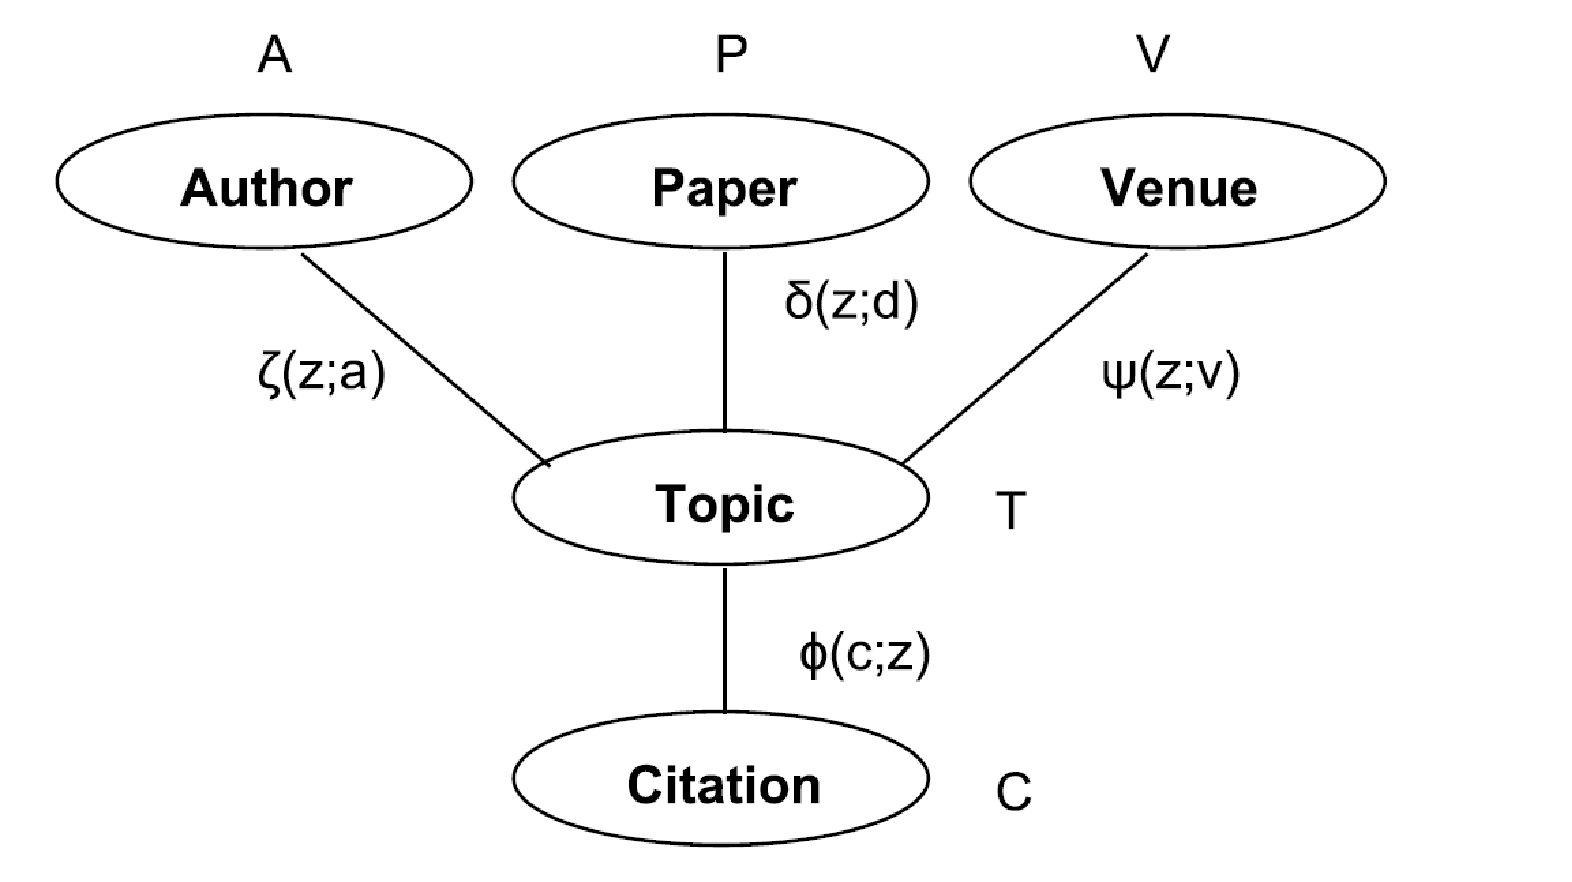
\includegraphics[width=1\linewidth]{images/mymodel.pdf}\\}
% The process of generating an academic document is as follows: for each citation in that document, firstly sample a topic $\topic_k$ according to the distribution from paper\_topic distribution $\delta(\topic ; \paper)$ or author\_topic distribution $\zeta(\topic ; \authorvar)$ or venue\_topic distribution $\psi(\topic ; \venue)$  based on the document type. Then, draw a citation $\citationvar$ from the sampled topic distribution $\phi(:;\topic_k)$ in topic\_citation distribution $\phi(\citationvar;\topic)$.
% \end{multicols}

\lstinputlisting[linerange=7-11]{./import_src/src1.txt}
\lstinputlisting[linerange=13-15]{./import_src/src1.txt}
}

\vspace{-0.5em}
%%%%%%%%%%%%%%%%%%%%%%%%%%%%%%%%%%%%%%%%%%%%%%%%%%%%%%%%%%%%%%%%%%%%%%%%%%%
\headerbox{with- Methods}{name=with,column=1,span=2,row=0,below=results}{
  %%%%%%%%%%%%%%%%%%%%%%%%%%%%%%%%%%%%%%%%%%%%%%%%%%%%%%%%%%%%%%%%%%%%%%%%%%%%%%
\lstinputlisting[linerange=1-5]{./import_src/src2.txt}
}

\vspace{-0.5em}
%%%%%%%%%%%%%%%%%%%%%%%%%%%%%%%%%%%%%%%%%%%%%%%%%%%%%%%%%%%%%%%%%%%%%%%%%%%
\headerbox{Mutable Data \& Field Type Refinement}{name=refine,column=1,span=2,row=0,below=with}{
  %%%%%%%%%%%%%%%%%%%%%%%%%%%%%%%%%%%%%%%%%%%%%%%%%%%%%%%%%%%%%%%%%%%%%%%%%%%%%%
\lstinputlisting[linerange=7-10]{./import_src/src2.txt}
}
\vspace{-0.5em}

%%%%%%%%%%%%%%%%%%%%%%%%%%%%%%%%%%%%%%%%%%%%%%%%%%%%%%%%%%%%%%%%%%%%%%%%%%%
\headerbox{More in the paper}{name=more,column=1,span=2,row=0,below=refine}{
  %%%%%%%%%%%%%%%%%%%%%%%%%%%%%%%%%%%%%%%%%%%%%%%%%%%%%%%%%%%%%%%%%%%%%%%%%%%%%%
 
\noindent{\centering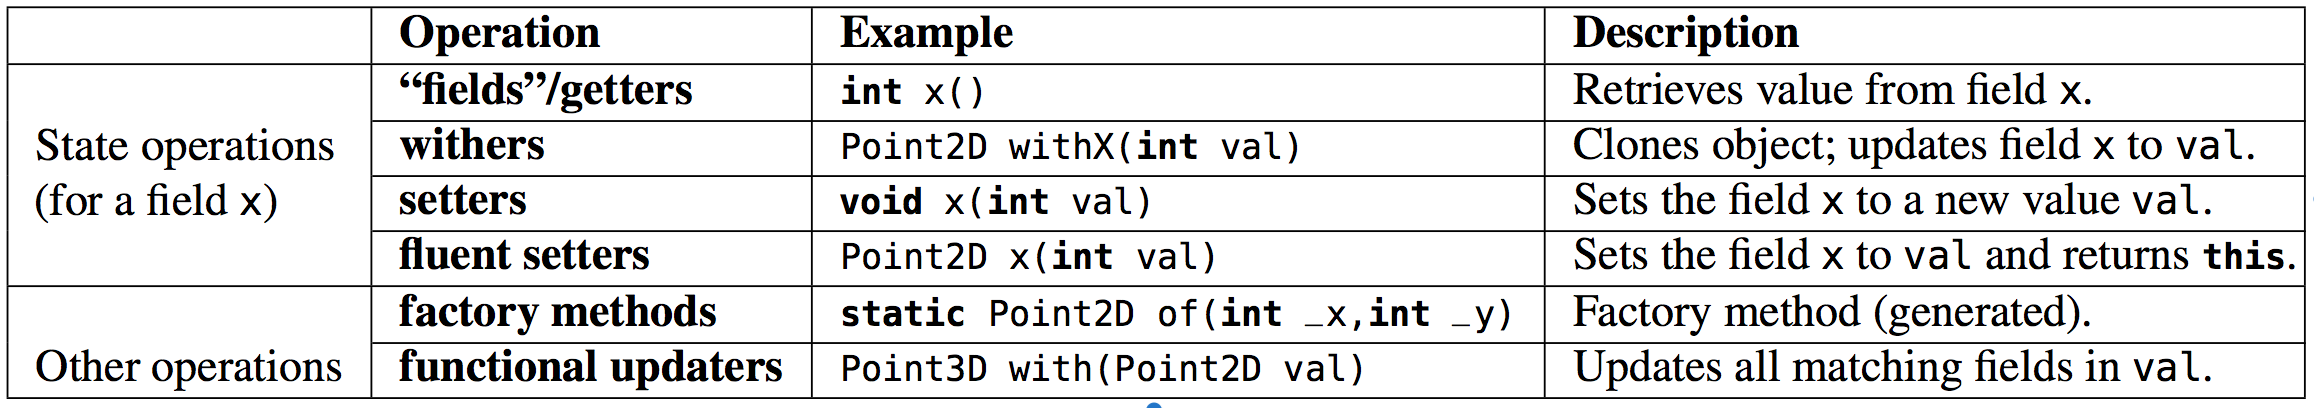
\includegraphics[width=0.95\linewidth]{table.png}\\}

\begin{multicols}{2}
\noindent{\centering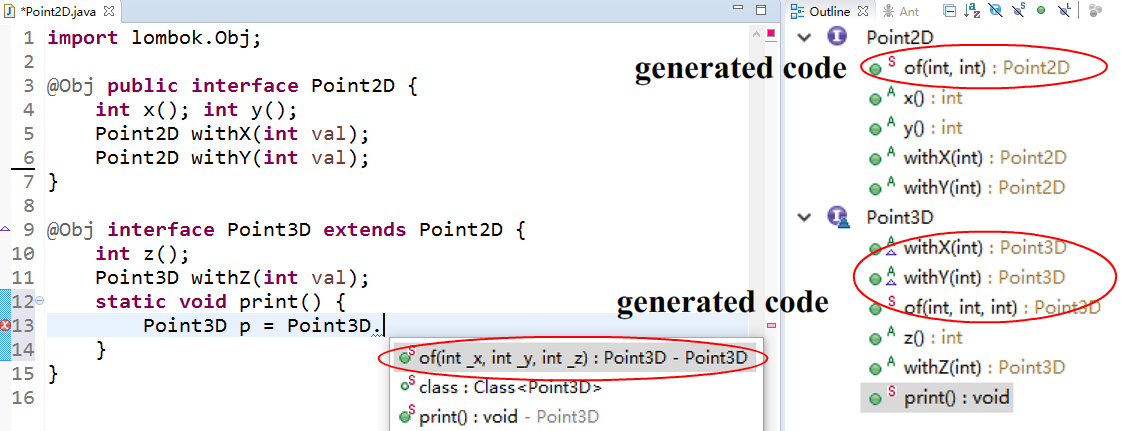
\includegraphics[width=1.15\linewidth]{pdfs/screenshot4.png}\\}
\begin{itemize}\compresslist
\item Techniques for field type refinement.
\item Formalization and proofs.
\item Case studies and applications.
    \small{\newline
    % \begin{itemize}\compresslist
    % \item The Expression Problem
    % \item Embedded DSLs with Fluent Interfaces
    % \item A Maze Game
    % \item Refactoring an Interpreter
    % \end{itemize}
    [The Expression Problem]\newline
    [Embedded DSLs with Fluent Interfaces]\newline
    [A Maze Game]\newline
    [Refactoring an Interpreter] 
    }
\end{itemize}
\end{multicols}
}

% %%%%%%%%%%%%%%%%%%%%%%%%%%%%%%%%%%%%%%%%%%%%%%%%%%%%%%%%%%%%%%%%%%%%%%%%%%%%%%%
%   \headerbox{Results(Partial)}{name=result2,column=1, span=2, below=more}{
% %%%%%%%%%%%%%%%%%%%%%%%%%%%%%%%%%%%%%%%%%%%%%%%%%%%%%%%%%%%%%%%%%%%%%%%%%%%%%%
% 2nd case study, embedding DSLs with our implementation of 
% fluent interfaces is quite straightforward:
% \lstinputlisting[linerange=17-18]{./import_src/src1.txt}
% }

% %%%%%%%%%%%%%%%%%%%%%%%%%%%%%%%%%%%%%%%%%%%%%%%%%%%%%%%%%%%%%%%%%%%%%%%%%%%%%%%
%   \headerbox{Limitations}{name=limitations,column=1,below=result2,above=bottom}{
% %%%%%%%%%%%%%%%%%%%%%%%%%%%%%%%%%%%%%%%%%%%%%%%%%%%%%%%%%%%%%%%%%%%%%%%%%%%%%%
% \begin{itemize}\compresslist
% \item Current implementation only realizes ejc version.
% \item Generics is not fully supported.
% \item Separate compilation is an experimental feature with current Lombok.
% \end{itemize}
% \vspace{0.3em}
%   }

%%%%%%%%%%%%%%%%%%%%%%%%%%%%%%%%%%%%%%%%%%%%%%%%%%%%%%%%%%%%%%%%%%%%%%%%%%%%%%
  \headerbox{Acknowledgments}{name=acknowledge,column=1, span=2, below=more}{
%%%%%%%%%%%%%%%%%%%%%%%%%%%%%%%%%%%%%%%%%%%%%%%%%%%%%%%%%%%%%%%%%%%%%%%%%%%%%%
This work is sponsored by the Hong Kong Research Grant Council Early Career 
Scheme project number 27200514. The first and second authors are supported by 
the SIG PAC student travel grant.
  }

%%%%%%%%%%%%%%%%%%%%%%%%%%%%%%%%%%%%%%%%%%%%%%%%%%%%%%%%%%%%%%%%%%%%%%%%%%%%%%
  \headerbox{Contacts}{name=acknowledge,column=1,span=2,below=acknowledge,above=bottom}{
%%%%%%%%%%%%%%%%%%%%%%%%%%%%%%%%%%%%%%%%%%%%%%%%%%%%%%%%%%%%%%%%%%%%%%%%%%%%%%
\noindent \textbf{The University of Hong Kong} \\
Yanlin Wang, Haoyuan Zhang, Bruno C. d. S. Oliveira: \emph{\{ylwang,hyzhang,bruno\}@cs.hku.hk} \\
\newline
\textbf{Victoria University of Wellington} \\
Marco Servetto: \emph{marco.servetto@ecs.vuw.ac.nz}
}

\end{poster}
\end{document}

